\documentclass[10pt,a4paper]{article}

\usepackage[margin=1.5cm, top=1.6cm, bottom=1.6cm]{geometry}
\usepackage{fontspec}
\usepackage{xcolor}
\usepackage{tikz}
\usetikzlibrary{mindmap,trees,shapes.geometric,arrows.meta,positioning,shadows}
\usepackage{tcolorbox}
\tcbuselibrary{breakable,skins}
\usepackage{booktabs}
\usepackage{tabularx}
\usepackage{enumitem}
\usepackage{hyperref}
\usepackage{fancyhdr}
\usepackage{multicol}

% Color Palette
\definecolor{navy}{HTML}{1B365D}
\definecolor{teal}{HTML}{007A87}
\definecolor{coral}{HTML}{D94F3D}
\definecolor{amber}{HTML}{D9822B}
\definecolor{plum}{HTML}{6B4C9A}
\definecolor{slate}{HTML}{4A5568}
\definecolor{lightgray}{HTML}{F4F6F9}
\definecolor{softblue}{HTML}{EBF3FA}
\definecolor{softred}{HTML}{FDF0EE}
\definecolor{softgreen}{HTML}{EDF7F1}
\definecolor{forestgreen}{HTML}{2E7D32}

\hypersetup{
    colorlinks=true,
    linkcolor=navy,
    urlcolor=teal
}

\pagestyle{fancy}
\fancyhf{}
\lhead{\small\textcolor{slate}{\textbf{ICAIDES 2026 Q\&A Prep} --- Paper ID 1571359798}}
\rhead{\small\textcolor{slate}{Fatih Jawwad Al Mumtaz (UNIDA Gontor)}}
\cfoot{\small\textcolor{slate}{\thepage}}
\renewcommand{\headrulewidth}{0.4pt}

% Custom Boxes
\newtcolorbox{qabox}[3][]{
  enhanced,
  breakable,
  colback=white,
  colframe=#2,
  coltitle=white,
  fonttitle=\bfseries\small,
  title={#3},
  boxrule=0.8pt,
  arc=3pt,
  left=6pt, right=6pt, top=5pt, bottom=5pt,
  before skip=6pt, after skip=6pt,
  #1
}

\newtcolorbox{infobox}[2][]{
  enhanced,
  breakable,
  colback=#2!6,
  colframe=#2,
  boxrule=0.6pt,
  arc=3pt,
  left=7pt, right=7pt, top=5pt, bottom=5pt,
  before skip=5pt, after skip=5pt,
  #1
}

\begin{document}

% ==================== HEADER BANNER ====================
\begin{tcolorbox}[
  enhanced,
  colback=navy,
  colframe=navy,
  coltext=white,
  arc=4pt,
  left=10pt, right=10pt, top=8pt, bottom=8pt
]
\begin{center}
{\Large\bfseries ICAIDES 2026 --- Research Mindmap \& Q\&A Defense Guide}\\[4pt]
{\normalsize\textit{Localizing INT8 Quantization Collapse in EfficientNet-B0 for Edge Poultry Disease Detection}}\\[6pt]
\small
\textbf{Presenter:} Fatih Jawwad Al Mumtaz \quad|\quad
\textbf{Session:} Parallel Session VII, Room A (Online) \quad|\quad
\textbf{Paper ID:} 1571359798\\[2pt]
\textbf{Schedule:} Friday, 13 Nov 2026, 15:30--15:45 WIB (Jakarta GMT+7) \quad|\quad
\textbf{Moderator:} Teny Handhayani
\end{center}
\end{tcolorbox}

% ==================== 30-SECOND ELEVATOR PITCH ====================
\begin{infobox}{teal}
\textbf{\textcolor{teal}{30-Second Summary (Hafalkan untuk Pembuka / Jika Diminta Ringkas):}}\\
``Our work evaluates whether lightweight CNNs---MobileNetV2, ShuffleNetV2, and EfficientNet-B0---survive INT8 post-training quantization on a Raspberry Pi 5 for farm-level poultry disease detection. First, we audited the published 8,770-image FecalFed benchmark and found 617 near-duplicate pairs including 94 byte-identical test-train leaks, so we built a clean 8,153-image split. Second, we found that dynamic INT8 preserves MobileNetV2 and ShuffleNetV2 within 1 percentage point, but collapses EfficientNet-B0 from 98.55\% to 10.42\%---a near-single-class predictor---and we localized this failure to per-tensor quantization of depthwise layers with extreme channel-range imbalance. Third, on Raspberry Pi 5, dynamic INT8 is actually 1.93--2.80$\times$ slower than FP32 due to runtime dequantize overhead, while static per-channel QDQ recovers EfficientNet-B0 to 94.56\% at 13.50 ms---yet ShuffleNetV2 FP32 remains faster and more accurate at 6.19 ms and 97.69\%.''
\end{infobox}

% ==================== SECTION 1: MINDMAP ====================
\section*{\textcolor{navy}{1. Research Mindmap (Peta Konsep Penelitian)}}
\vspace{-4pt}
\begin{center}
\resizebox{\linewidth}{!}{%
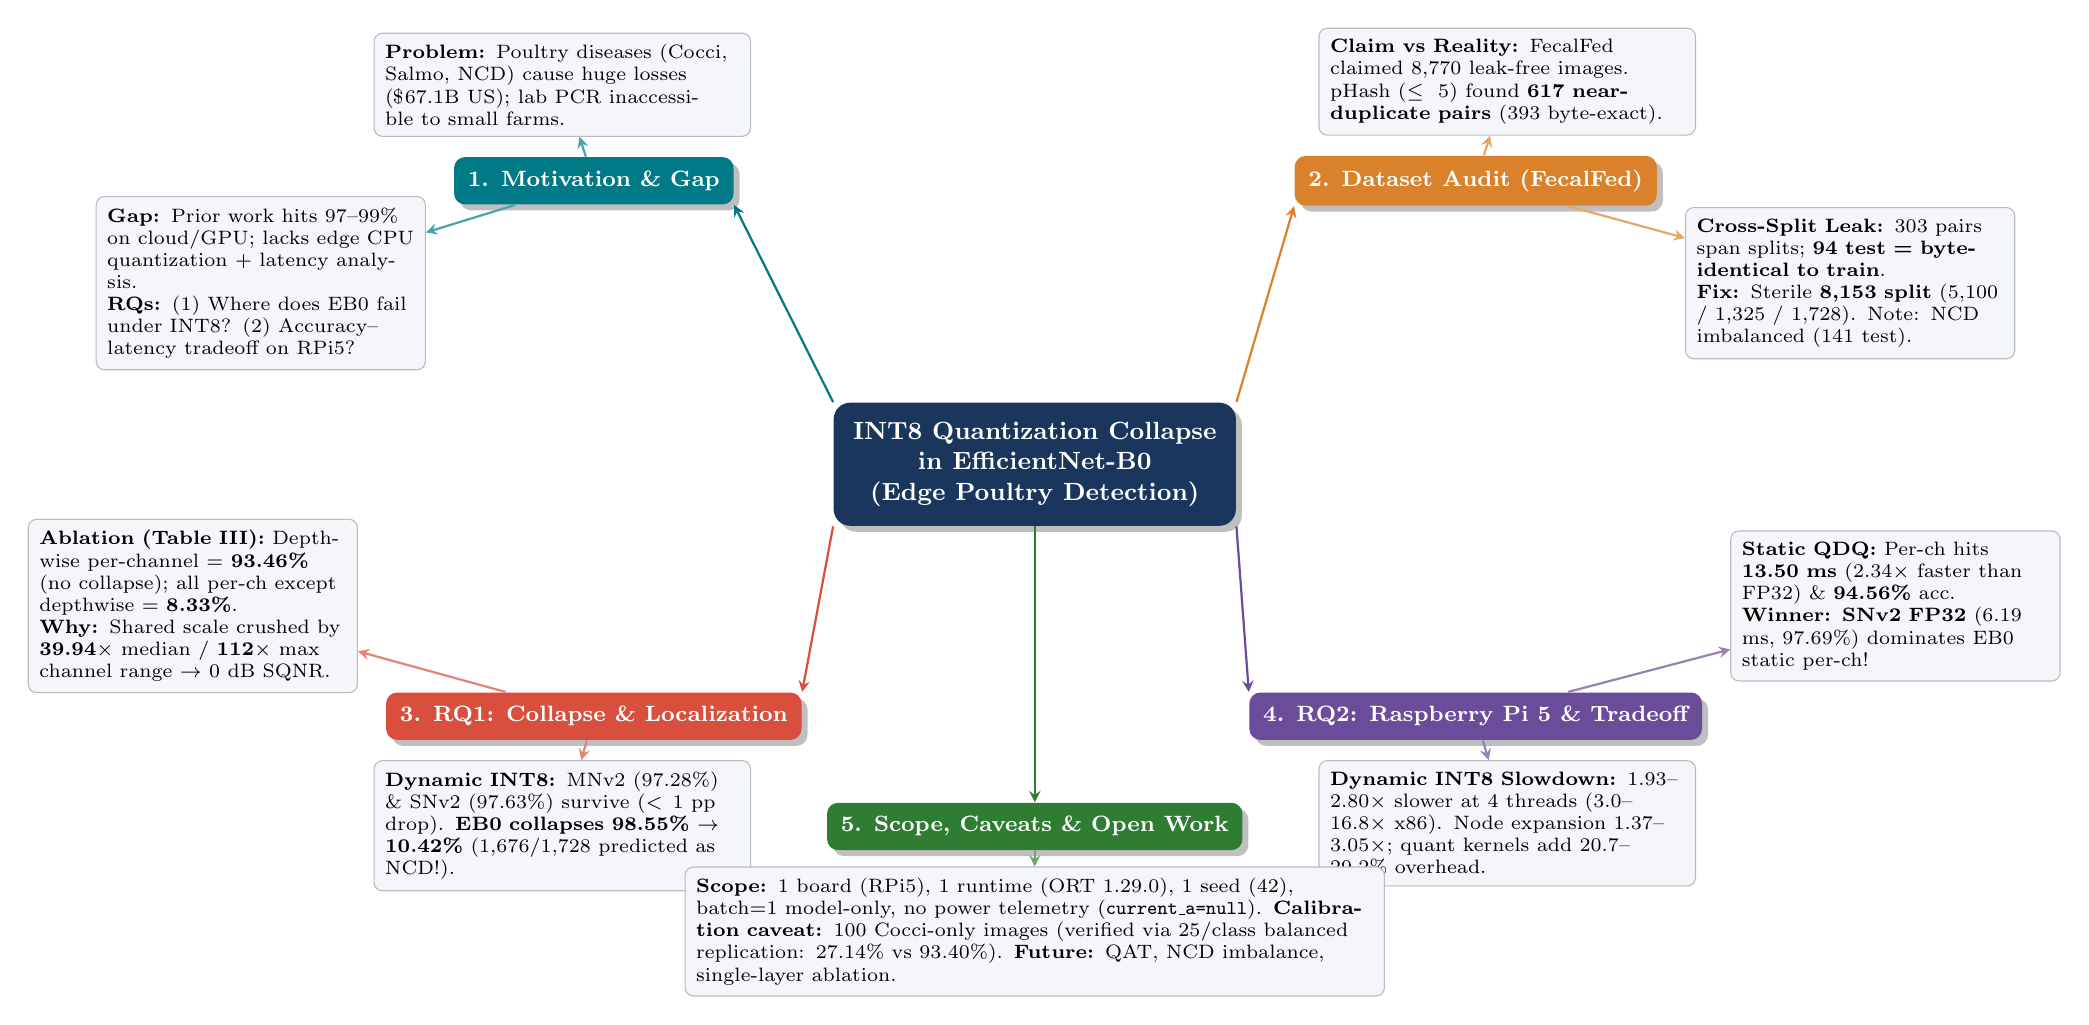
\begin{tikzpicture}[
  every node/.style={font=\scriptsize, align=center},
  root/.style={rectangle, rounded corners=6pt, fill=navy, text=white, font=\small\bfseries, inner sep=7pt, drop shadow},
  branch/.style={rectangle, rounded corners=4pt, text=white, font=\footnotesize\bfseries, inner sep=5pt, drop shadow},
  leaf/.style={rectangle, rounded corners=3pt, fill=lightgray, draw=slate!40, inner sep=4pt, text width=4.5cm, align=left},
  edge/.style={->, >=stealth, thick}
]

% Central Node
\node[root] (center) at (0,0) {INT8 Quantization Collapse\\in EfficientNet-B0\\(Edge Poultry Detection)};

% Branch 1: Top-Left (Motivation & Gap)
\node[branch, fill=teal] (b1) at (-5.6, 3.6) {1. Motivation \& Gap};
\node[leaf, above=0.25cm of b1, xshift=-0.4cm] (l1a) {
  \textbf{Problem:} Poultry diseases (Cocci, Salmo, NCD) cause huge losses (\$67.1B US); lab PCR inaccessible to small farms.
};
\node[leaf, left=0.35cm of b1, yshift=-1.3cm, text width=3.9cm] (l1b) {
  \textbf{Gap:} Prior work hits 97--99\% on cloud/GPU; lacks edge CPU quantization + latency analysis.\\
  \textbf{RQs:} (1) Where does EB0 fail under INT8? (2) Accuracy--latency tradeoff on RPi5?
};
\draw[edge, teal] (center.north west) -- (b1.south east);
\draw[edge, teal!70] (b1) -- (l1a);
\draw[edge, teal!70] (b1) -- (l1b);

% Branch 2: Top-Right (Dataset Audit)
\node[branch, fill=amber] (b2) at (5.6, 3.6) {2. Dataset Audit (FecalFed)};
\node[leaf, above=0.25cm of b2, xshift=0.4cm] (l2a) {
  \textbf{Claim vs Reality:} FecalFed claimed 8,770 leak-free images. pHash ($\le 5$) found \textbf{617 near-duplicate pairs} (393 byte-exact).
};
\node[leaf, right=0.35cm of b2, yshift=-1.3cm, text width=3.9cm] (l2b) {
  \textbf{Cross-Split Leak:} 303 pairs span splits; \textbf{94 test = byte-identical to train}.\\
  \textbf{Fix:} Sterile \textbf{8,153 split} (5,100 / 1,325 / 1,728). Note: NCD imbalanced (141 test).
};
\draw[edge, amber] (center.north east) -- (b2.south west);
\draw[edge, amber!70] (b2) -- (l2a);
\draw[edge, amber!70] (b2) -- (l2b);

% Branch 3: Bottom-Left (RQ1: Collapse & Root Cause)
\node[branch, fill=coral] (b3) at (-5.6, -3.2) {3. RQ1: Collapse \& Localization};
\node[leaf, below=0.25cm of b3, xshift=-0.4cm] (l3a) {
  \textbf{Dynamic INT8:} MNv2 (97.28\%) \& SNv2 (97.63\%) survive ($<1$ pp drop). \textbf{EB0 collapses 98.55\% $\to$ 10.42\%} (1,676/1,728 predicted as NCD!).
};
\node[leaf, left=0.35cm of b3, yshift=1.4cm, text width=3.9cm] (l3b) {
  \textbf{Ablation (Table III):} Depthwise per-channel = \textbf{93.46\%} (no collapse); all per-ch except depthwise = \textbf{8.33\%}.\\
  \textbf{Why:} Shared scale crushed by \textbf{39.94$\times$} median / \textbf{112$\times$} max channel range $\to$ 0 dB SQNR.
};
\draw[edge, coral] (center.south west) -- (b3.north east);
\draw[edge, coral!70] (b3) -- (l3a);
\draw[edge, coral!70] (b3) -- (l3b);

% Branch 4: Bottom-Right (RQ2: Edge RPi5 & Tradeoff)
\node[branch, fill=plum] (b4) at (5.6, -3.2) {4. RQ2: Raspberry Pi 5 \& Tradeoff};
\node[leaf, below=0.25cm of b4, xshift=0.4cm] (l4a) {
  \textbf{Dynamic INT8 Slowdown:} 1.93--2.80$\times$ slower at 4 threads (3.0--16.8$\times$ x86). Node expansion 1.37--3.05$\times$; quant kernels add 20.7--29.2\% overhead.
};
\node[leaf, right=0.35cm of b4, yshift=1.4cm, text width=3.9cm] (l4b) {
  \textbf{Static QDQ:} Per-ch hits \textbf{13.50 ms} (2.34$\times$ faster than FP32) \& \textbf{94.56\%} acc.\\
  \textbf{Winner:} \textbf{SNv2 FP32} (6.19 ms, 97.69\%) dominates EB0 static per-ch!
};
\draw[edge, plum] (center.south east) -- (b4.north west);
\draw[edge, plum!70] (b4) -- (l4a);
\draw[edge, plum!70] (b4) -- (l4b);

% Branch 5: Bottom-Center (Scope & Open Work)
\node[branch, fill=forestgreen] (b5) at (0, -4.6) {5. Scope, Caveats \& Open Work};
\node[leaf, below=0.2cm of b5, text width=8.6cm] (l5) {
  \textbf{Scope:} 1 board (RPi5), 1 runtime (ORT 1.29.0), 1 seed (42), batch=1 model-only, no power telemetry (\texttt{current\_a=null}). \textbf{Calibration caveat:} 100 Cocci-only images (verified via 25/class balanced replication: 27.14\% vs 93.40\%). \textbf{Future:} QAT, NCD imbalance, single-layer ablation.
};
\draw[edge, forestgreen] (center.south) -- (b5.north);
\draw[edge, forestgreen!70] (b5) -- (l5);

\end{tikzpicture}%
}
\end{center}

\newpage

% ==================== SECTION 2: CHEAT SHEET ====================
\section*{\textcolor{navy}{2. Key Numbers Cheat Sheet (Angka Wajib Hafal)}}

\begin{multicols}{2}
\begin{tcolorbox}[colback=softblue, colframe=navy, title=\textbf{A. Dataset \& Models}, fonttitle=\small\bfseries, boxrule=0.6pt]
\small
\begin{itemize}[leftmargin=*, itemsep=2pt]
  \item \textbf{Original FecalFed:} 8,770 images (7,016 train / 1,754 test)
  \item \textbf{pHash Audit ($\le 5$):} 617 near-duplicate pairs (393 byte-exact)
  \item \textbf{Cross-split leaks:} 303 pairs (147 test--train, 54 test--val, 102 train--val); \textbf{94 test} byte-identical to train
  \item \textbf{Sterile Split:} \textbf{8,153} images (5,100 train / 1,325 val / 1,728 test)
  \item \textbf{NCD Class:} 417/5,100 train, 141/1,728 test (underrepresented)
  \item \textbf{Params (4-class):} SNv2 1.3M, MNv2 2.2M, EB0 4.0M
  \item \textbf{Size Reduction:} 3.3--3.7$\times$ smaller (e.g., EB0 15.3 $\to$ 4.16 MB)
\end{itemize}
\end{tcolorbox}

\begin{tcolorbox}[colback=softred, colframe=coral, title=\textbf{B. Accuracy \& Ablation (n = 1,728)}, fonttitle=\small\bfseries, boxrule=0.6pt]
\small
\begin{itemize}[leftmargin=*, itemsep=2pt]
  \item \textbf{FP32:} MNv2 97.92\%, SNv2 97.69\%, EB0 \textbf{98.55\%} (ONNX 98.50\%)
  \item \textbf{Dynamic INT8:} MNv2 97.28\% ($p=0.0455$), SNv2 97.63\% ($p=1.0$), EB0 \textbf{10.42\%} ($-88.13$ pp; 1,676/1,728 predicted NCD)
  \item \textbf{Static QDQ (EB0):} Per-tensor \textbf{9.32\%} vs Per-channel \textbf{94.56\%}
  \item \textbf{Balanced 25/class check:} Per-tensor \textbf{27.14\%} vs Per-channel \textbf{93.40\%}
  \item \textbf{Ablation C (Depthwise per-ch, rest per-tensor):} \textbf{93.46\%} (No collapse)
  \item \textbf{Ablation D (All per-ch EXCEPT depthwise):} \textbf{8.33\%} (Collapse!)
  \item \textbf{Ablation E vs F:} Depthwise FP32 = \textbf{97.16\%} vs SE FP32 = \textbf{12.44\%}
\end{itemize}
\end{tcolorbox}
\end{multicols}

\vspace{-6pt}
\begin{tcolorbox}[colback=softgreen, colframe=forestgreen, title=\textbf{C. SQNR, Channel Range \& Raspberry Pi 5 Latency (ORT 1.29.0, batch=1, t=4)}, fonttitle=\small\bfseries, boxrule=0.6pt]
\footnotesize
\resizebox{\linewidth}{!}{%
\begin{tabular}{@{}lcccccc@{}}
\toprule
\textbf{Model} & \textbf{DW Median P95/P5} & \textbf{DW SQNR (Per-Ten $\to$ Per-Ch)} & \textbf{RPi5 FP32 (t=4)} & \textbf{RPi5 Dyn INT8 (t=4)} & \textbf{Thread Scale (1$\to$4)} & \textbf{Quant Overhead} \\
\midrule
MobileNetV2 & 9.20$\times$ & 34.06 dB med (12.23 worst) & 14.23 ms & 39.83 ms (2.80$\times$ slower) & 2.33$\times$ vs 1.10$\times$ & 29.2\% \\
ShuffleNetV2 & 5.32$\times$ & 37.79 dB med & \textbf{6.19 ms} & 11.95 ms (1.93$\times$ slower) & 2.29$\times$ vs 1.14$\times$ & 20.7\% \\
EfficientNet-B0 & \textbf{39.94$\times$} (max 112$\times$) & \textbf{27.97 $\to$ 44.42 dB} (0 dB worst) & 31.56 ms & 64.39 ms (2.04$\times$ slower) & 2.20$\times$ vs 1.19$\times$ & 24.9\% \\
\bottomrule
\end{tabular}%
}
\vspace{4pt}
\small
\textbf{EB0 Static QDQ on RPi5 (t=4):} Static per-tensor = 13.63 ms (9.32\% acc); Static per-channel = \textbf{13.50 ms} (2.34$\times$ faster than FP32, \textbf{94.56\%} acc).
\end{tcolorbox}

% ==================== SECTION 3: Q&A BANK ====================
\section*{\textcolor{navy}{3. Anticipated Q\&A Bank (English, Clear \& Ready to Memorize)}}
\textit{\small Tips: Jawab langsung ke inti dalam 2--4 kalimat dulu (Direct Answer), baru sebutkan angka pendukungnya jika perlu. Jangan bertele-tele.}

\subsection*{\textcolor{teal}{Category A: Motivation, Novelty \& Contribution}}

\begin{qabox}{teal}{Q1. Depthwise separability and per-channel quantization are already known (e.g., Sheng et al. 2018, Krishnamoorthi 2018). What is the novel contribution of your paper?}
\textbf{Answer:}
``We do not claim depthwise quantization sensitivity as a new theoretical discovery. Our contribution is empirical and practical in three ways: first, we expose and clean 617 near-duplicate leaks in the FecalFed benchmark; second, we present a controlled case study showing that under an identical PTQ pipeline, EfficientNet-B0 collapses completely while MobileNetV2 and ShuffleNetV2 survive, and we localize it to depthwise granularity; third, we characterize the real runtime bottleneck on Raspberry Pi 5, showing that dynamic INT8 is 2$\times$ slower than FP32 while ShuffleNetV2 FP32 actually dominates quantized EfficientNet-B0.''\\[3pt]
\textbf{Key Numbers:} 617 near-duplicates removed; EB0 10.42\% vs MNv2/SNv2 $>97\%$; RPi5 dynamic slowdown 1.93--2.80$\times$.
\end{qabox}

\begin{qabox}{teal}{Q2. Why focus on edge deployment on a Raspberry Pi 5 instead of cloud or smartphone inference?}
\textbf{Answer:}
``Smallholder poultry farms in rural areas often lack reliable internet connectivity for cloud inference and cannot afford GPU servers. A single-board computer like the Raspberry Pi 5 enables low-cost, offline, on-farm screening right at the coop, while keeping data local.''\\[3pt]
\textbf{Key Context:} Prior work (Dhungana 99.12\%, Tasdelen 97.1\%) targets cloud/GPU; our work bridges the farm-level deployment gap.
\end{qabox}

\begin{qabox}{teal}{Q3. Why did you choose MobileNetV2, ShuffleNetV2, and EfficientNet-B0 specifically?}
\textbf{Answer:}
``These three are standard, widely deployed lightweight CNN families with different architectural blocks: MobileNetV2 uses inverted residuals, ShuffleNetV2 uses channel shuffle, and EfficientNet-B0 adds Squeeze-and-Excitation with compound scaling. Comparing them under the exact same pipeline lets us isolate which architectural features survive INT8 quantization on CPU.''\\[3pt]
\textbf{Key Numbers:} Parameter counts (4-class): ShuffleNetV2 1.3M, MobileNetV2 2.2M, EfficientNet-B0 4.0M.
\end{qabox}

\subsection*{\textcolor{amber}{Category B: Dataset Audit \& Methodology}}

\begin{qabox}{amber}{Q4. Why did you audit the FecalFed dataset, and how did you choose pHash with Hamming distance $\le 5$?}
\textbf{Answer:}
``The FecalFed paper claimed 8,770 rigorously deduplicated, leak-free images. We audited that claim using perceptual hashing (pHash) with a conservative threshold of Hamming distance $\le 5$ to catch both exact copies and near-duplicates such as slight crops or re-encodings. Even at this conservative threshold, we found 617 near-duplicate pairs, including 94 test images that were byte-for-byte identical to training images.''\\[3pt]
\textbf{Key Numbers:} 8,770 $\to$ 617 pairs (393 byte-exact, 303 cross-split: 147 test--train, 54 test--val, 102 train--val) $\to$ sterile 8,153 split.
\end{qabox}

\begin{qabox}{amber}{Q5. Why did you split train/val before deduplication, and why prioritize keeping test > val > train?}
\textbf{Answer:}
``We kept the publisher's test split intact first so our evaluation remains comparable to the benchmark's intended test distribution. When removing one image from each duplicate pair, prioritizing test > val > train ensured zero cross-split leakage while preserving as much of the 1,754-image test set as possible---98\% of it (1,728 images) was retained.''\\[3pt]
\textbf{Key Numbers:} Removed 513 train, 78 val, 26 test = 617 total; final split 5,100 / 1,325 / 1,728.
\end{qabox}

\begin{qabox}{amber}{Q6. Newcastle Disease (NCD) is underrepresented (141 test images). Does that affect your conclusions?}
\textbf{Answer:}
``Yes, NCD is smaller (417 train, 141 test), which is why we report both overall accuracy and macro-F1 / balanced accuracy. In FP32, all three models still achieve over 97\% macro-F1, showing they learn NCD well. Under dynamic INT8, however, EfficientNet-B0 collapses to predicting NCD for 1,676 out of 1,728 images, dropping macro-F1 to 7.49\%.''\\[3pt]
\textbf{Key Numbers:} EB0 FP32 macro-F1 98.22\% (bal. acc 98.03\%) vs INT8 macro-F1 7.49\% (bal. acc 26.89\%).
\end{qabox}

\subsection*{\textcolor{coral}{Category C: Quantization Collapse \& Root Cause}}

\begin{qabox}{coral}{Q7. Why does EfficientNet-B0 collapse specifically into predicting Newcastle Disease (100\% NCD recall)?}
\textbf{Answer:}
``When depthwise weights are quantized per-tensor, channels with narrow weight ranges are crushed to near-zero or constant values---our SQNR audit shows 0 dB in the worst channels. This destroys class-discriminative spatial features, so the network's output logits become dominated by static biases and activations, pushing nearly all inputs (1,676 of 1,728) into a single default class---in this case, NCD.''\\[3pt]
\textbf{Key Numbers:} Per-class INT8 recall: Coccidiosis 2.27\%, Healthy 4.76\%, Salmonella 0.54\%, NCD 100\%.
\end{qabox}

\begin{qabox}{coral}{Q8. Your static QDQ calibration used 100 Coccidiosis-only images! Doesn't that bias invalidate your static QDQ results?}
\textbf{Answer:}
``That is a great catch, and we state it upfront as a diagnostic caveat. To test whether calibration skew caused the collapse, we ran a balanced 25-images-per-class replication on a retrained model. Balanced calibration lifted per-tensor accuracy from 9.32\% to 27.14\%, so the collapse still persisted, while per-channel stayed at 93.40\%. This confirms that quantization granularity, not calibration skew, drives the collapse.''\\[3pt]
\textbf{Key Numbers:} Retrained FP32 98.15\%; balanced static per-tensor 27.14\% vs balanced static per-channel 93.40\%.
\end{qabox}

\begin{qabox}{coral}{Q9. How can you be sure depthwise layers---and not Squeeze-and-Excitation (SE) layers---cause the collapse?}
\textbf{Answer:}
``Our selective per-family ablation in Table III directly isolates this. When we keep only depthwise layers per-channel and everything else per-tensor (Config C), accuracy recovers to 93.46\% with no collapse. Conversely, when we quantize everything per-channel except depthwise (Config D), accuracy collapses to 8.33\%. Leaving SE layers in FP32 (Config F) still collapses to 12.44\%, whereas leaving depthwise in FP32 (Config E) achieves 97.16\%.''\\[3pt]
\textbf{Key Proof:} Depthwise per-channel granularity is both necessary and sufficient to avoid collapse in this setup.
\end{qabox}

\begin{qabox}{coral}{Q10. Why do MobileNetV2 and ShuffleNetV2 survive the exact same dynamic INT8 pipeline?}
\textbf{Answer:}
``Because their depthwise layers have much tighter channel-wise weight ranges. Our range audit shows EfficientNet-B0's depthwise layers have a median P95/P5 channel-range ratio of 39.94$\times$ (and up to 112$\times$ in the worst layer), compared to only 9.20$\times$ in MobileNetV2 and 5.32$\times$ in ShuffleNetV2. As a result, MobileNetV2's worst depthwise channel stays at 12.23 dB SQNR, whereas EfficientNet-B0 drops to 0 dB.''\\[3pt]
\textbf{Key Numbers:} Median depthwise per-tensor SQNR: EB0 16.67 dB, MNv2 34.06 dB, SNv2 37.79 dB.
\end{qabox}

\subsection*{\textcolor{plum}{Category D: Edge Deployment, Runtime \& Shipping Choice}}

\begin{qabox}{plum}{Q11. INT8 is supposed to be faster than FP32. Why is dynamic INT8 2--16$\times$ SLOWER in your experiments?}
\textbf{Answer:}
``Dynamic INT8 is slower here because of how ONNX Runtime 1.29.0 executes dynamic quantization on CPU. Each convolution expands into \texttt{DynamicQuantizeLinear}, \texttt{ConvInteger}, \texttt{Mul}, and \texttt{Cast}, growing the graph node count by 1.37--3.05$\times$. Our kernel profiling on Raspberry Pi 5 shows that these extra quantization kernels add 20.7--29.2\% runtime overhead, and dynamic INT8 barely scales across 4 threads (1.10--1.19$\times$ vs 2.20--2.33$\times$ for FP32).''\\[3pt]
\textbf{Key Proof:} Switching to \emph{static} QDQ removes runtime activation quantization and makes EB0 2.34$\times$ faster than FP32 (13.50 ms vs 31.53 ms).
\end{qabox}

\begin{qabox}{plum}{Q12. Does INT8 quantization reduce memory (RAM) usage during inference on Raspberry Pi 5?}
\textbf{Answer:}
``It shrinks the model file size on disk by 3.3--3.7$\times$ (for example, EfficientNet-B0 drops from 15.3 MB to 4.16 MB), which helps storage and OTA updates. However, at batch size 1 on Raspberry Pi 5, runtime RSS memory barely changes---around 99--108 MB for MobileNetV2 and 111--112 MB for ShuffleNetV2---because runtime buffers and ONNX Runtime overhead dominate.''
\end{qabox}

\begin{qabox}{plum}{Q13. Why did you measure model-only latency instead of end-to-end latency (including image loading and preprocessing)?}
\textbf{Answer:}
``We measured model-only latency to isolate the compute and kernel behavior of the neural network architectures and quantization schemes without confounding it with Python I/O, JPEG decoding, or camera capture latency. We clearly state this as a scope boundary, and in production, preprocessing would add a fixed overhead on top of model inference.''
\end{qabox}

\begin{qabox}{plum}{Q14. So if I am building a poultry farm device tomorrow, which model should I actually deploy?}
\textbf{Answer:}
``Deploy \textbf{ShuffleNetV2 in FP32}. On Raspberry Pi 5 at 4 threads, ShuffleNetV2 FP32 runs in 6.19 ms with 97.69\% accuracy. It is more than twice as fast AND more accurate than static per-channel INT8 EfficientNet-B0 (13.50 ms, 94.56\%). Since FP32 accuracy across all three models differs by less than 0.86 percentage points, ShuffleNetV2 FP32 gives the best practical accuracy--latency tradeoff without quantization risk.''
\end{qabox}

\subsection*{\textcolor{forestgreen}{Category E: Limitations, Threats to Validity \& Future Work}}

\begin{qabox}{forestgreen}{Q15. Did you try Quantization-Aware Training (QAT) or Cross-Layer Equalization (CLE) to fix EfficientNet-B0?}
\textbf{Answer:}
``Not yet---this study specifically characterizes post-training quantization (PTQ) because PTQ requires no retraining pipeline and is the first choice for many edge developers. Cross-layer equalization and QAT are well-known remedies for channel range imbalance and are natural next steps for future work.''
\end{qabox}

\begin{qabox}{forestgreen}{Q16. Your experiments use only one seed (42), one board (RPi 5), and one runtime (ORT 1.29.0). How generalizable are your results?}
\textbf{Answer:}
``We intentionally scope our claims to this measured stack---one board, one runtime build, one dataset, and one training seed---rather than claiming universal hardware generality. However, we did replicate the static QDQ diagnostic on a retrained model with balanced calibration and observed the same collapse behavior, and our x86 reference confirmed the dynamic INT8 slowdown pattern.''
\end{qabox}

\begin{qabox}{forestgreen}{Q17. What about power or energy consumption on the Raspberry Pi 5? Farms often run on solar or battery.}
\textbf{Answer:}
``We attempted to read onboard current telemetry, but \texttt{current\_a} returned null on this Raspberry Pi 5 setup, so we report energy measurement as a limitation. We did monitor die temperature (44--56$^\circ$C) and confirmed zero thermal throttling across all 12 benchmark configurations.''
\end{qabox}

\begin{qabox}{forestgreen}{Q18. Why didn't you test single-layer ablation to prove which exact depthwise layer triggers the collapse?}
\textbf{Answer:}
``Our ablation was conducted at the operator-family level (all depthwise vs all SE vs all pointwise), which already proves that depthwise granularity is necessary and sufficient. Identifying whether one specific severe layer---like the 480-channel layer with 112$\times$ range ratio---triggers the collapse alone is a concrete hypothesis we leave for single-layer ablation in future work.''
\end{qabox}

% ==================== SECTION 4: BONUS SURVIVAL PLAYBOOK ====================
\section*{\textcolor{navy}{4. Bonus: Q\&A Survival Playbook (Biar Gak Panik Besok)}}

\begin{multicols}{2}
\begin{infobox}{navy}
\textbf{\textcolor{navy}{5 Golden Phrases Saat Ditanya Hal Susah:}}
\begin{enumerate}[leftmargin=*, itemsep=3pt, topsep=2pt]
  \item \textbf{Jika tidak tahu / di luar scope:}\\
  \textit{``That is a great question. We did not measure that in this current scope, as we focused on [X], so it remains an open direction for future work.''}
  \item \textbf{Jika dikritik soal limitasi (mis. 1 seed / no QAT):}\\
  \textit{``Yes, we agree and explicitly acknowledge that limitation in Section V. Our goal here was to isolate the PTQ failure mode first.''}
  \item \textbf{Jika kurang jelas mendengar pertanyaan (Zoom):}\\
  \textit{``Thank you for the question. Could you kindly repeat the last part so I can address it accurately?''}
  \item \textbf{Jika butuh waktu 3 detik untuk berpikir:}\\
  \textit{``Thank you, that is an interesting point. Let me answer that in two parts...''}
  \item \textbf{Menutup jawaban dengan rapi:}\\
  \textit{``...I hope that answers your question. Thank you.''}
\end{enumerate}
\end{infobox}

\begin{infobox}{coral}
\textbf{\textcolor{coral}{Checklist Teknis Sebelum Besok (15:30 WIB):}}
\begin{itemize}[leftmargin=*, itemsep=3pt, topsep=2pt]
  \item \textbf{Masuk Zoom 15 menit lebih awal (15:15 WIB):}\\
  Link: \texttt{https://bit.ly/ZoomICAIDES2026}\\
  Meeting ID: \texttt{823 1206 1206} \quad|\quad Passcode: \texttt{Untar67}
  \item \textbf{Urutan Tampil:} Kamu presenter \textbf{ke-2} di Parallel Session VII Room A (setelah Iswadi Hasyim Rosma).
  \item \textbf{Cek Minor Typo di Slide (jika masih bisa diedit):}
  \begin{itemize}[leftmargin=*, itemsep=1pt]
    \item Slide 1 subtitle tertulis \textit{``Raspberry Pi 3''} (padahal paper \& slide lain \textbf{Raspberry Pi 5}).
    \item Slide 1 tertulis \textit{``ICAIDES 2025 / NOVEMBER 2025''} (konferensi resminya \textbf{ICAIDES 2026 / November 2026}).
  \end{itemize}
  \item \textbf{Buka PDF Paper / Slide di layar kedua} agar kalau ditanya angka tabel, tinggal lirik tanpa panik!
\end{itemize}
\end{infobox}
\end{multicols}

\end{document}
